\documentclass{article}
\usepackage[a4paper, tmargin=1in, bmargin=1in]{geometry}
\usepackage[utf8]{inputenc}
\usepackage{graphicx}
\usepackage{parskip}
\usepackage{pdflscape}
\usepackage{listings}
\usepackage{amsmath}

\usepackage{float}
\usepackage{hyperref}
% \usepackage{titlesec}
\usepackage{fp}
\usepackage{siunitx}

\newcommand{\ConverFracToDecimal}{%
    \renewcommand*{\frac}[2]{%
        \FPdiv\Result{##1}{##2}%
        \num[round-mode=places,round-precision=4]{\Result}%
    }%
}%


\newcommand{\ra}{$\rightarrow$}

\newenvironment{question}[2][Question]{\begin{trivlist}
  \item[\hskip \labelsep {\bfseries #1}\hskip \labelsep {\bfseries #2:}]}{\end{trivlist}}
\newenvironment{answer}[2][Answer]{\begin{trivlist}
  \item[\hskip \labelsep {\bfseries #1}\hskip \labelsep {\bfseries #2:}]}{\end{trivlist}}


\title{EE 302 : Control System Home Assignment}
\author{
  Arka Sadhu - 140070011\\
  Sudeep Salgia - 14D070011\\
  Parth Kothari - 14D070019\\
}

\date{\today}

\begin{document}
\maketitle
\begin{answer} a
  The freebody diagrams are as follows:
  \begin{figure}[H]
    \centering
    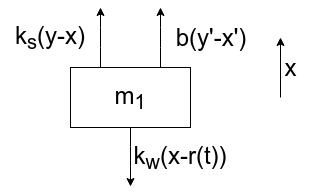
\includegraphics[scale=0.5]{images/m1_fbd}
    \caption{Free body diagram of m1}
    \label{fig:1}
  \end{figure}
  \begin{figure}[H]
    \centering
    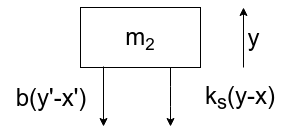
\includegraphics[scale=0.5]{images/m2_fbd}
    \caption{Free body diagram of m2}
    \label{fig:2}
  \end{figure}
  \begin{equation}
    \label{eq:1}
    m_1\ddot{x} = k_s(y-x) + b(\dot{y} - \dot{x}) + k_w(r(t) - x)
  \end{equation}
  \begin{equation}
    \label{eq:2}
    m_2\ddot{y} = k_s(x-y) + b(\dot{x} - \dot{y}) 
  \end{equation}
  Converting (\ref{eq:1}) to the Laplace Domain and taking initial conditions as 0. We get
  \begin{equation}
    \label{eq:3}
    m_1s^2X(s) = k_s[Y(s) - X(s)] + bs[Y(s) - X(s)] + k_w[R(s) - X(s)]
  \end{equation}
  
  Rearranging the terms we get
  \begin{equation}
    \label{eq:4}
    [m_1 s^2 + bs + (k_s+k_w)]X(s) = [bs + k_s]Y(s) + k_wR(s)
  \end{equation}

  Converting (\ref{eq:2}) to the Laplace Domain and taking initial conditions as 0. We get
  \begin{equation}
    \label{eq:5}
    m_2s^2 Y(s) = k_s[X(s) - Y(s)] + bs[X(s) - Y(s)]
  \end{equation}
  
  Rearranging the terms we get
  \begin{equation}
    \label{eq:6}
    [m_2s^2 + k_s + bs]Y(s) = [k_s + bs]X(s)
  \end{equation}
  Put X(s) from (\ref{eq:6}) into (\ref{eq:4}) we get
  % $$[m_1s^2 + bs + (k_s + k_w)]X(s) = [bs + k_s]Y(s) + k_wR(s)$$
  $$\frac{[m_1s^2 + bs + (k_s + k_w)]}{[k_s + bs]}[m_2s^2 + k_s + bs - (k_s + bs)^2]Y(s) = k_w(k_s+ bs)R(s)$$
  $$\frac{Y(s)}{R(s)} = \frac{ k_w(k_s+ bs)}{[m_1s^2 + bs + (k_s + k_w)][m_2s^2 + k_s + bs] - (k_s + bs)^2]}$$
\end{answer}

\begin{answer}b
  $$\dot{p} = Ap + Br$$
  $$y = Cp + Dr$$
  Here
  \[
    p = \begin{bmatrix}
      x \\
      \dot{x}\\
      y\\
      \dot{y}
    \end{bmatrix}
  \]
  Making use of (\ref{eq:1}) and (\ref{eq:2}) to get the second and fourth row of A. We get
  $$A = \left(\begin{array}{cccc} 0 & 1 & 0 & 0\\ -\frac{k_{s} + k_{w}}{m_{1}} & -\frac{b}{m_{1}} & \frac{k_{s}}{m_{1}} & \frac{b}{m_{1}}\\ 0 & 0 & 0 & 1\\ \frac{k_{s}}{m_{2}} & \frac{b}{m_{2}} & -\frac{k_{s}}{m_{2}} & -\frac{b}{m_{2}} \end{array}\right)$$
  
  $$B = \left(\begin{array}{c} 0\\ \frac{k_{w}}{m_{1}}\\ 0\\ 0 \end{array}\right)$$
  \[
    C =
    \begin{bmatrix}
      0 & 0 & 1 & 0
    \end{bmatrix}
  \]
  $$ D = 0$$
\end{answer}

\begin{answer}c
  From state space to Transfer function we use
  $$G(s) = C(sI - A)^{-1}B$$
  We get
  $$G(s) = \frac{k_{w}\, \left(k_{s} + b\, s\right)}{m_{1}\, m_{2}\, s^4 + \left(b\, m_{1} + b\, m_{2}\right)\, s^3 + \left(k_{s}\, m_{1} + k_{s}\, m_{2} + k_{w}\, m_{2}\right)\, s^2 + b\, k_{w}\, s + k_{s}\, k_{w}}$$
  which is the same as that in part(a).

\end{answer}

\begin{answer}d
  The controller canonical form of a state space model is given by
  \[
    A_{ccf} =
    \begin{bmatrix}
      -a_3 & -a_2 & -a_1 & -a_0\\
      1 & 0 & 0 & 0\\
      0 & 1 & 0 & 0\\
      0 & 0 & 1 & 0
    \end{bmatrix}
  \]
  where the characteristic equation is
  $$s^4 + a_3s^3 + a_2 s^2 + a_1 s + a_0 = 0$$
  Controller Canonical Form of the matrix is
  $$A_{ccf} = \left(\begin{array}{cccc} -\frac{b\, m_{1} + b\, m_{2}}{m_{1}\, m_{2}} & -\frac{k_{s}\, m_{1} + k_{s}\, m_{2} + k_{w}\, m_{2}}{m_{1}\, m_{2}} & -\frac{b\, k_{w}}{m_{1}\, m_{2}} & -\frac{k_{s}\, k_{w}}{m_{1}\, m_{2}}\\ 1 & 0 & 0 & 0\\ 0 & 1 & 0 & 0\\ 0 & 0 & 1 & 0 \end{array}\right)$$
\end{answer}

\begin{answer}e
  From \ref{eq:1} we have
  $$m_1\ddot{x} = k_s(y-x) + b(\dot{y} - \dot{x}) + k_w(r(t) - x) - f_{act}$$
  Rearranging the terms we get
  \begin{equation}
    \label{eq:7}
    \ddot{x} + \frac{b}{m_1}(\dot{x} - \dot{y}) + \frac{k_s}{m_1}(x - y) + \frac{k_w}{m_1}x = \frac{k_w}{m_1}r - \frac{f_{act}}{m_1}
  \end{equation}
  From \ref{eq:2} we have
  $$m_2\ddot{y} = k_s(x-y) + b(\dot{x} - \dot{y})$$
  Rearranging the terms we get
  \begin{equation}
    \label{eq:8}
    \ddot{y} + \frac{b}{m_2}(\dot{y} - \dot{x}) + \frac{k_s}{m_2}(y - x) = \frac{f_{act}}{m_2}
  \end{equation}

\end{answer}
\begin{answer}f
  $$\dot{p} = Ap + B_1r + B_2f_{act}$$
  $$ y = Cp + D_1r + D_2f_{act}$$

  A will remain the same as in (c) and $B_1$ will be same as $B$.
  Using \ref{eq:7} and \ref{eq:8} we get
  \[
    B_2 =
    \begin{bmatrix}
      0\\
      \frac{-1}{m_1}\\
      0\\
      \frac{1}{m_2}
    \end{bmatrix}
  \]
  Both $D_1$ and $D_2$ turn out to be 0.  
\end{answer}
\begin{answer}g
  The solution with $f_{act} = 0$ is
  $$p(t) = e^{At}p(0) + \int_0^t e^{A(t-\tau)}B_1r(\tau)d\tau$$
  Impulse response with initial condition $p(0) = 0$ is
  $$p(t) = \int_0^t e^{A(t-\tau)}B_1r(\tau)d\tau = \int_0^t e^{A(t-\tau)}B_1\delta(\tau)d\tau$$
  $$p(t) = e^{At}B_1$$
  The response of the system with $r = 0$ and initial condition $B_1$ is
  $$p(t) = e^{At}p(0) = e^{At}B_1$$
  Since $D_1$ and $D_2$ are zero, we get
  $$y = Cp$$
  To prove that the impulse responses are the same, it suffices to show that the $p(t)$ is the same for both the cases. \\
  Hence we have proved that the impulse response of the system with $f_{act} = 0$ and initial condition $p(0)=0$ is the same as response of the system with $f_{act} = 0$ and $r=0$ and initial condition $B_1$
\end{answer}

\begin{answer}h
  To get peak overshoot $M=2.5\%$ and settling time $t_s = 0.39sec$, using second order approximation, we get the poles to be placed as
  $$p_1 = -11.7949 -j 10.0450$$
  $$p_2 = -11.7949 -j 10.0450$$
  % asdf
  The other two poles to be placed are at $$p_3 = -60$$ $$p_4 = -100$$

  The required transfer function would have the characteristic polynomial as
  $$G_{required}(s) = s^4 + 183.5898s^3 + 10014.389691s^2 + 179942.2705616s^1 + 1440130.14606$$

  From this we get the required A matrix in canonical form as
  $$A_{reqd\_canonical} = \left(\begin{array}{cccc} - 183.5898 & - 10014.38969101 & -179942.270561600 & -1440130.14606 \\ 1 & 0 & 0 & 0\\ 0 & 1 & 0 & 0\\ 0 & 0 & 1 & 0 \end{array}\right)$$

  The current A matrix represented in canonical form is
  $$A_{ccf} = \left(\begin{array}{cccc} -\frac{b\, m_{1} + b\, m_{2}}{m_{1}\, m_{2}} & -\frac{k_{s}\, m_{1} + k_{s}\, m_{2} + k_{w}\, m_{2}}{m_{1}\, m_{2}} & -\frac{b\, k_{w}}{m_{1}\, m_{2}} & -\frac{k_{s}\, k_{w}}{m_{1}\, m_{2}}\\ 1 & 0 & 0 & 0\\ 0 & 1 & 0 & 0\\ 0 & 0 & 1 & 0 \end{array}\right)$$
  On replacing the corresponding values $k_w = 1000000$, $k_s = 130000$, $b = 9800$, $m_1 = 80$, $m_2 = 1500$,
  $$A_{ccf} = \left(\begin{array}{cccc} -129.0333 & -14211.667 & -81666.6667 & -1083333.3333 \\ 1 & 0 & 0 & 0\\ 0 & 1 & 0 & 0\\ 0 & 0 & 1 & 0 \end{array}\right)$$

  So we find $K_{reqd\_canonical}$ as
  $$K_{reqd\_canonical} = A_{ccf} - A_{reqd\_canonical} = \left(\begin{array}{cccc} 54.5564667 & -4197.27697 & 98275.6038 & 356796.81272 \end{array}\right)$$

  Now we convert this K to our current form, by multiplying $T^{-1}$ where $T$ is the transformation matrix required to transform the state space to control canonical form.
  $$K = K_{reqd\_canonical}T^{-1} = \ConverFracToDecimal \left(\begin{array}{cccc} \frac{2903961887049187}{8589934592} & - \frac{1026821118672775}{274877906944} & \frac{5884533665195789}{137438953472} & \frac{1620827538137813}{137438953472} \end{array}\right)$$
  The new A is given as
  $$A_{state\_feedback} =\ConverFracToDecimal \left(\begin{array}{cccc} 0 & 1 & 0 & 0\\ - \frac{2721065680764325}{274877906944} & - \frac{744124921344795}{4398046511104} & \frac{2375159761655579}{1099511627776} & \frac{4748366851461461}{17592186044416}\\ 0 & 0 & 0 & 1\\ - \frac{610054959817109}{4398046511104} & \frac{5079892796380467}{562949953421312} & - \frac{8107211986451043}{70368744177664} & - \frac{4051939713247113}{281474976710656} \end{array}\right)$$
\end{answer}

\begin{answer}i
  The observer canonical form is given by $$ A_{obs} = \left(\begin{array}{cccc} -\frac{b\, m_{1} + b\, m_{2}}{m_{1}\, m_{2}} & 1 & 0 & 0\\ -\frac{k_{s}\, m_{1} + k_{s}\, m_{2} + k_{w}\, m_{2}}{m_{1}\, m_{2}} & 0 & 1 & 0\\ -\frac{b\, k_{w}}{m_{1}\, m_{2}} & 0 & 0 & 1\\ -\frac{k_{s}\, k_{w}}{m_{1}\, m_{2}} & 0 & 0 & 0 \end{array}\right) $$.  

  On replacing the corresponding values $k_w = 1000000$, $k_s = 130000$, $b = 9800$, $m_1 = 80$, $m_2 = 1500$, we get 

  $$ A_obs =  \ConverFracToDecimal \left(\begin{array}{cccc} - \frac{3871}{30} & - \frac{42635}{3} & - \frac{245000}{3} & - \frac{3250000}{3}\\ 1 & 0 & 0 & 0\\ 0 & 1 & 0 & 0\\ 0 & 0 & 1 & 0 \end{array}\right) $$ 


  
\end{answer}
\begin{answer}j
The observer design problem can be treated in the same way as the pole placement problem with for the system matrix in observer canonical form and for this specific case, we need to place the poles at $ -60, -100, -300 $ and $ -400$. Hence the required transfer function is $$G(s) = s^4 + 860s^3 + 23800s^2 + 23400000s^1 + 720000000$$ 
and hence the corresponding required $A$ matrix in the observer canonical form is $$A_{reqd\_observer} = \left(\begin{array}{cccc} - 860 & 1 & 0 & 0 \\ -23800 & 0 & 1 & 0\\ -23400000 & 0 & 0 & 1\\ -720000000 & 0 & 0 & 0 \end{array}\right)$$

Thus using the same procedure as adopted in the case for pole placement problem, we get $L_{reqd\_observer}$ as
  $$L_{reqd\_observer} = A_{ocf} - A_{reqd\_observer} = \left(\begin{array}{cccc} 730.966 & 223788.333 & 23318333.333 & 718916666.666 \end{array}\right)^{T}$$

  Now we convert this L to our current form, by premultiplying $T^{-1}$ where $T$ is the transformation matrix required to transform the state space to observer canonical form $$L = T^{-1} L_{reqd\_observer} = \left(\begin{array}{cccc} 13662.845 & -620000.4096 & 730.967 & 129469.268 \end{array}\right)^{T}$$

  The new $A$ is hence given as 

$$ A_{state_feedback} =\ConverFracToDecimal  \left(\begin{array}{cccc} 0 & 1 & - \frac{1877807075575657}{137438953472} & 0\\ -14125 & - \frac{245}{2} & \frac{1334930402236375}{2147483648} & \frac{245}{2}\\ 0 & 0 & - \frac{21929}{30} & 1\\ \frac{260}{3} & \frac{98}{15} & - \frac{4451508011532871}{34359738368} & - \frac{98}{15} \end{array}\right) $$
\end{answer}

\begin{answer}l
  The performance index to be minimized is
  $$J = \int_0^\infty 2y^2(t) + f_{act}^2(t)dt$$
  This can be solved using the theory of Symmetric Root Locus, which provides solution of minimization the following performance index.
  $$J = \int_0^\infty \rho y^2(t) + f_{act}^2(t)dt$$
  where $f_{act} = -Kp$.\\
  The optimal value of K is that which places the closed-loop poles at the stable roots (those in the LHP) of the symmetric root-locus (SRL) equation
  $$1 + \rho G_0(-s)G_0(s) = 0$$
  where
  $$G_0(s) = \frac{Y(s)}{f_{act}(s)} = C(sI - A)^{-1}B_2$$
\end{answer}



\end{document}

